% chktex-file 44

\documentclass[a4paper,11pt]{article}
\usepackage[utf8]{inputenc}
\usepackage[russian]{babel}
\usepackage{geometry}
\usepackage{amsthm}
\usepackage[dvipsnames]{xcolor}
\usepackage{framed}
\usepackage{booktabs}
\usepackage{array}
\usepackage{amssymb}
\usepackage{adjustbox}
\usepackage{makecell}
\usepackage{float}
\usepackage{graphicx}
\graphicspath{{../}}
\usepackage{amsmath}
\usepackage{physics}
\usepackage{hyperref}
\usepackage{color}
\usepackage{listings}

\definecolor{shadecolor}{RGB}{245,245,247}
\geometry{left=2cm, right=2cm, top=2cm, bottom=2cm}


\title{Модель №.4. \\ Магнитные колебания. \\ Связанные маятники }
\author{Ким В.Р., Вишневский С.А \\ Группа M3207 }
\date{}

\theoremstyle{definition}
\newtheorem*{task}{Задание}\setlength{\parindent}{0pt}

\newenvironment{solution}
{\begin{shaded}\textbf{Решение:}\par\setlength{\parindent}{0pt}}
{\end{shaded}}

\newenvironment{answer}
{\par\noindent\textbf{Ответ:} }
{\par}

\definecolor{codegreen}{rgb}{0,0.6,0}
\definecolor{codegray}{rgb}{0.5,0.5,0.5}
\definecolor{codepurple}{rgb}{0.58,0,0.82}
\definecolor{backcolour}{rgb}{0.95,0.95,0.92}

\lstdefinelanguage{MyPython}{
    language=Python,
    morekeywords={np, plt, self, cos, sin},
    sensitive=true,
}
\lstdefinestyle{mystyle}{
    backgroundcolor=\color{backcolour},
    commentstyle=\color{codegreen},
    keywordstyle=\color{magenta},
    numberstyle=\tiny\color{codegray},
    stringstyle=\color{codepurple},
    basicstyle=\ttfamily\footnotesize,
    breakatwhitespace=false,
    breaklines=true,
    captionpos=b,
    keepspaces=true,
    numbers=left,
    numbersep=5pt,
    showspaces=false,
    showstringspaces=false,
    showtabs=false,
    tabsize=2,
    columns=fullflexible,
}

\lstset{style=mystyle}

\begin{document}
\maketitle

\begin{task}
    Два одинаковых математических маятника, связанных пружиной с коэффициентом 
    жёсткости \(k\) на расстоянии \(L_1\) от точки крепления маятников. 
    Точки крепления обоих связанных маятников находятся на одном уровне. 
    Оба математических маятника имеют одинаковые длины подвеса \(L\) и массы \(m\) 
    (см. Рис.). 
    Сила сопротивления для каждого маятника прямо пропорциональна скорости. 
    Коэффициент затухания каждого маятника равен \(\beta\). Для заданных начальных 
    отклонений построить графики зависимостей углов и скоростей от времени 
    для каждого маятника. Найти нормальные частоты. 
    Параметры должны задаваться.

    \begin{figure}[H]
        \centering
        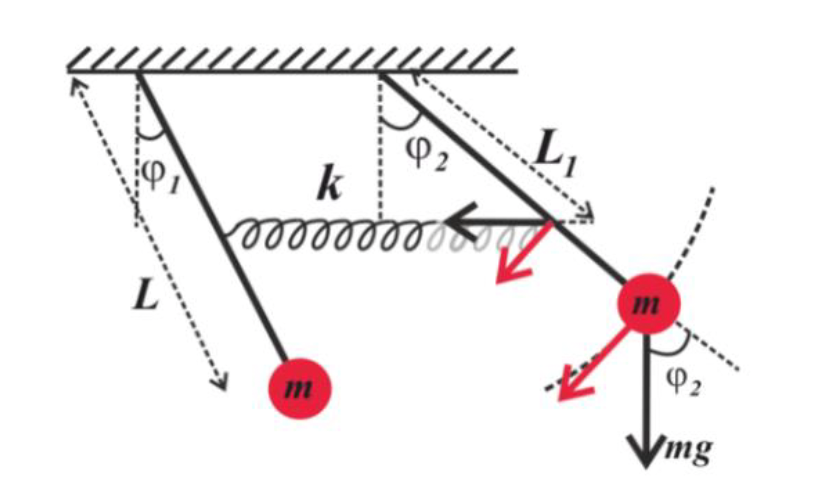
\includegraphics[width=0.5\textwidth]{task}\label{fig:figure}
    \end{figure}

\end{task}


\section*{Введение и постановка задачи}
Рассматривается система двух идентичных математических маятников, подвешенных на равной высоте, соединённых 
пружиной с коэффициентом жёсткости \( k \). Пружина прикреплена к маятникам на расстоянии \( L_1 \) от точки 
их крепления. Каждый маятник имеет длину \( L \) и массу \( m \). Для каждого маятника учитывается сила 
затухания, пропорциональная скорости, с коэффициентом \(\beta\). Целью задачи является построение графиков 
зависимости угловых отклонений и угловых скоростей от времени, а также определение нормальных частот системы.



\section*{Математический маятник: определения и базовые уравнения}
\textbf{Математический маятник} --- идеализированная модель, в которой масса сосредоточена в точке, а подвес 
считается нерастяжимым и безмассовым. Обобщённой координатой является угол отклонения \(\phi\) от вертикального 
направления (положения равновесия).

Для малых колебаний (при условии \(\sin \phi \approx \phi\)) уравнение движения выводится из закона 
сохранения момента импульса:
\[
\frac{d\vec{M}}{dt} = \vec{N},
\]
где \(\vec{M}\) --- момент импульса, а \(\vec{N}\) --- суммарный момент сил, действующих на систему.

Приводя это уравнение к скалярной форме для колебаний вокруг точки крепления, получаем:
\[
\ddot{\phi} + \omega_0^2 \phi = 0,
\]
где \(\omega_0 = \sqrt{\frac{g}{L}}\) --- собственная (естественная) частота свободного маятника, 
а \(g\) --- ускорение свободного падения.

При наличии затухающего сопротивления, пропорционального скорости, уравнение принимает вид:
\[
\ddot{\phi} + 2\beta\dot{\phi} + \omega_0^2 \phi = 0.
\]
Здесь \(\beta\) --- коэффициент затухания, отражающий диссипативные процессы в системе.



\subsection*{Система двух связанных маятников}
При рассмотрении двух маятников, связанных пружиной, следует учитывать взаимодействие, возникающее 
из-за разности их углов. Обозначим:
\[
\phi_1(t), \phi_2(t)
\]
--- углы отклонения первого и второго маятников соответственно.

В отсутствие затухания, уравнения движения можно записать следующим образом:
\begin{gather}
    \ddot{\phi}_1 + \omega_0^2 \phi_1 - \kappa^2 (\phi_2 - \phi_1) = 0,\\
    \ddot{\phi}_2 + \omega_0^2 \phi_2 + \kappa^2 (\phi_2 - \phi_1) = 0.\\
\end{gather}
Здесь введён параметр связи \(\kappa\), который определяется через жёсткость пружины и геометрию 
системы. Часто встречается соотношение:
\[
\kappa^2 = \frac{k L_1^2}{mL^2}.
\]
Знак в членах, содержащих \(\kappa^2(\phi_2 - \phi_1)\), отражает то, что пружинная сила стремится 
уменьшить разницу углов маятников.

С учётом затухания уравнения дополняются членами, пропорциональными скорости:
\begin{gather}
    \ddot{\phi}_1 + 2\beta\dot{\phi}_1 + \omega_0^2 \phi_1 - \kappa^2 (\phi_2 - \phi_1) = 0,\\
    \ddot{\phi}_2 + 2\beta\dot{\phi}_2 + \omega_0^2 \phi_2 + \kappa^2 (\phi_2 - \phi_1) = 0.\\
\end{gather}



\subsection*{Преобразование в нормальные координаты и нормальные моды}
Для упрощения анализа системы удобно ввести нормальные координаты:
\[
\xi_1 = \phi_1 + \phi_2, \quad \xi_2 = \phi_2 - \phi_1.
\]
Путём суммирования и вычитания исходных уравнений движения (без затухания для чистоты рассуждения) 
получаем:
\begin{gather*}
    \ddot{\xi}_1 + \omega_0^2 \xi_1 = 0,\\
    \ddot{\xi}_2 + \left(\omega_0^2 + 2\kappa^2\right) \xi_2 = 0.\\
\end{gather*}
Таким образом, система сводится к двум независимым колебательным уравнениям с нормальными частотами:
\[
\Omega_{n1} = \omega_0 = \sqrt{\frac{g}{L}}, \quad \Omega_{n2} = \sqrt{\omega_0^2 + 2\kappa^2} = \sqrt{\frac{g}{L} + \frac{2kL_1^2}{mL^2}}.
\]

Решения для нормальных координат имеют вид:
\begin{gather*}
    \xi_1(t) = \Phi_{01}\cos\left(\Omega_{n1}t+\varphi_{01}\right),\\
    \xi_2(t) = \Phi_{02}\cos\left(\Omega_{n2}t+\varphi_{02}\right),\\
\end{gather*}
где \(\Phi_{01}, \Phi_{02}\) --- амплитуды, а \(\varphi_{01}, \varphi_{02}\) --- начальные фазы, 
определяемые начальными условиями.

Переход обратно к углам маятников осуществляется по формулам:
\[
\phi_1 = \frac{\xi_1+\xi_2}{2}, \quad \phi_2 = \frac{\xi_1-\xi_2}{2}.
\]
В результате получаем общее решение для углов:
\begin{gather*}
    \phi_1(t) = \frac{1}{2}\left[\Phi_{01}\cos\left(\Omega_{n1}t+\varphi_{01}\right)+\Phi_{02}\cos\left(\Omega_{n2}t+\varphi_{02}\right)\right],\\
    \phi_2(t) = \frac{1}{2}\left[\Phi_{01}\cos\left(\Omega_{n1}t+\varphi_{01}\right)-\Phi_{02}\cos\left(\Omega_{n2}t+\varphi_{02}\right)\right].\\
\end{gather*}



\subsection*{Режимы колебаний}
В зависимости от начальных условий в системе могут возникать различные режимы колебаний:

\begin{enumerate}
    \item \textbf{Синфазное колебание:} Если задать начальные условия так, что \(\Phi_{02}=0\), то
    \[
    \phi_1(t)=\phi_2(t)=\frac{\Phi_{01}}{2}\cos\left(\Omega_{n1}t+\varphi_{01}\right).
    \]
    Оба маятника движутся синхронно с частотой \(\Omega_{n1} = \omega_0\).

    \item \textbf{Противофазное колебание:} Если задать начальные условия так, что \(\Phi_{01}=0\), то
    \[
    \phi_1(t)=\frac{\Phi_{02}}{2}\cos\left(\Omega_{n2}t+\varphi_{02}\right),\quad
    \phi_2(t)=-\frac{\Phi_{02}}{2}\cos\left(\Omega_{n2}t+\varphi_{02}\right).
    \]
    Маятники движутся с частотой \(\Omega_{n2}\), но в противоположных фазах.

    \item \textbf{Суперпозиция нормальных мод (биения):} При возбуждении обеих нормальных мод, например, 
    если только один маятник изначально отклонён, решение для первого маятника может записываться как
    \[
    \phi_1(t)=\frac{\phi_1(0)}{2}\left[\cos\left(\Omega_{n1}t\right)+\cos\left(\Omega_{n2}t\right)\right].
    \]
    Применяя тригонометрическую формулу для суммы косинусов, получаем:
    \[
    \phi_1(t)=\phi_1(0)\cos\left(\frac{\Omega_{n1}+\Omega_{n2}}{2}t\right)
    \cos\left(\frac{\Omega_{n2}-\Omega_{n1}}{2}t\right).
    \]
    Здесь быстрые колебания с частотой \(\frac{\Omega_{n1}+\Omega_{n2}}{2}\) амплитудно модулированы медленной 
    огибающей с частотой \(\frac{\Omega_{n2}-\Omega_{n1}}{2}\) --- эффект биений. При слабой связи разность 
    частот невелика, а период биений оценивается как
    \[
    T_{\textnormal{биений}} \approx \frac{2\pi}{\Omega_{n2}-\Omega_{n1}}.
    \]
\end{enumerate}



\subsection*{Учет затухания в системе}
В реальных системах затухание приводит к экспоненциальному уменьшению амплитуд. Сила затухания для каждого 
маятника пропорциональна его скорости, поэтому к уравнениям движения добавляется член \(2\beta\dot{\phi}\). 
Итоговые уравнения с учетом затухания имеют вид:
\begin{gather}
    \ddot{\phi}_1 + 2\beta\dot{\phi}_1 + \omega_0^2 \phi_1 - \kappa^2 (\phi_2 - \phi_1) = 0,\\
    \ddot{\phi}_2 + 2\beta\dot{\phi}_2 + \omega_0^2 \phi_2 + \kappa^2 (\phi_2 - \phi_1) = 0.\\
\end{gather}
Эти уравнения описывают, как затухание влияет на динамику системы, уменьшая амплитуду колебаний с течением времени.



\subsection*{Итоговая схема моделирования и интерпретация результатов}
При численной реализации модели выполняются следующие этапы:
\begin{itemize}
    \item \textbf{Инициализация параметров:} вводятся значения \(m\), \(L\), \(L_1\), \(k\), \(\beta\), \(g\) 
    и начальные условия для \(\phi_1\) и \(\phi_2\).
    \item \textbf{Формулировка системы ОДУ:} записываются уравнения движения для \(\phi_1(t)\) и \(\phi_2(t)\) 
    с учетом затухания и пружинной связи.
    \item \textbf{Численное интегрирование:} для решения системы дифференциальных уравнений используются 
    численные методы (например, метод Рунге--Кутты).
    \item \textbf{Построение графиков:} полученные решения представляются в виде графиков зависимости углов 
    \(\phi_1(t)\), \(\phi_2(t)\) и их производных (угловых скоростей) от времени.
    \item \textbf{Определение нормальных частот:} на основании формул
    \[
    \Omega_{n1}=\sqrt{\frac{g}{L}}, \quad \Omega_{n2}=\sqrt{\frac{g}{L}+\frac{2kL_1^2}{mL^2}},
    \]
    вычисляются нормальные частоты системы, что позволяет дополнительно проанализировать режимы синфазных 
    и противофазных колебаний.
\end{itemize}


\section*{Моделирование}

\subsection*{1. Инициализация параметров}
\begin{equation}
  m,\ L,\ L_1,\ k,\ \beta\label{eq:equation2}
\end{equation}

\begin{lstlisting}[language=MyPython,label={lst:lstlisting3}]
    m = float(entry_m.get())          # mass of pendulums (kg)
    L = float(entry_L.get())          # length of pendulum string (m)
    L1 = float(entry_L1.get())        # distance from suspension point to spring attachment (m)
    k = float(entry_k.get())          # spring stiffness (N/m)
    beta = float(entry_beta.get())    # damping coefficient (kg/s)
\end{lstlisting}

\subsection*{2. Задание начальных условий}
\begin{equation}
  \phi_1(0),\ \phi_2(0),\ \dot{\phi}_1(0),\ \dot{\phi}_2(0),\ T\label{eq:equation}
\end{equation}

\begin{lstlisting}[language=MyPython,label={lst:lstlisting2}]
    phi1_0 = float(entry_phi1.get())  # initial angle of first pendulum (rad)
    phi2_0 = float(entry_phi2.get())  # initial angle of second pendulum (rad)

    v1_0 = float(entry_v1.get())      # initial angular velocity of first pendulum (rad/s)
    v2_0 = float(entry_v2.get())      # initial angular velocity of second pendulum (rad/s)

    t_max = float(entry_time.get())   # maximum simulation time (s)
\end{lstlisting}

\subsection*{3. Система уравнений движения}

Аналитическая запись:
\begin{align*}
  \ddot{\phi}_1 &+ \frac{\beta}{m} \dot{\phi}_1 + \bigl(\tfrac{g}{L} + \kappa^2\bigr)\phi_1 - \kappa^2 \phi_2 = 0, \\
  \ddot{\phi}_2 &+ \frac{\beta}{m} \dot{\phi}_2 + \bigl(\tfrac{g}{L} + \kappa^2\bigr)\phi_2 - \kappa^2 \phi_1 = 0, \\
  \kappa^2 &= \frac{k L_1^2}{m L^2}.
\end{align*}

\begin{lstlisting}[language=MyPython,label={lst:lstlisting}]
def system(y, t, m, L, L1, k, beta, g=9.81):
    phi1, v1, phi2, v2 = y
    K = k * L1**2 / (m * L**2)      # κ² = k L1² / (m L²)
    omega0_sq = g / L               # ω₀² = g / L
    dydt = [
        v1,
        -(beta/m)*v1 - (omega0_sq + K)*phi1 + K*phi2,
        v2,
        -(beta/m)*v2 - (omega0_sq + K)*phi2 + K*phi1
    ]
    return dydt
\end{lstlisting}

\subsection*{4. Численное интегрирование}

Аналитическая форма: решение системы ОДУ
\begin{equation}
  \frac{d\mathbf{y}}{dt} = \mathrm{system}(\mathbf{y}, t)\label{eq:equation3}
\end{equation}

\begin{lstlisting}[language=MyPython,label={lst:lstlisting4}]
    y0  = [phi1_0, v1_0, phi2_0, v2_0]
    sol = odeint(system, y0, t, args=(m, L, L1, k, beta))
    phi1, v1, phi2, v2 = sol[:,0], sol[:,1], sol[:,2], sol[:,3]
\end{lstlisting}

\subsection*{5. Построение графиков}

Аналитическая постановка: визуализация $\phi_i(t)$ и $\dot{\phi}_i(t)$ для $i=1,2$.

\begin{lstlisting}[language=MyPython,label={lst:lstlisting5}]
    # График углов
    ax1.plot(t, phi1, label='φ₁(t)')
    ax1.plot(t, phi2, label='φ₂(t)')
    ax1.set_xlabel('t, с')
    ax1.set_ylabel('φ, рад')
    ax1.legend()

    # График скоростей
    ax2.plot(t, v1, label='φ̇₁(t)')
    ax2.plot(t, v2, label='φ̇₂(t)')
    ax2.set_xlabel('t, с')
    ax2.set_ylabel('скорость, рад/с')
    ax2.legend()
\end{lstlisting}

%\subsection*{6. Вычисление нормальных частот}
%
%Аналитические формулы:
%\begin{align*}
%  \Omega_1 &= \sqrt{\frac{g}{L}}, \\
%  \Omega_2 &= \sqrt{\frac{g}{L} + 2\kappa^2}.
%\end{align*}
%
%\begin{lstlisting}[language=MyPython,label={lst:lstlisting6}]
%    Omega_n1 = np.sqrt(omega0_sq)           # Ω₁ = √(g/L)
%    Omega_n2 = np.sqrt(omega0_sq + 2*K)     # Ω₂ = √(g/L + 2κ²)
%    print(f"Нормальные частоты: Ω₁={Omega_n1:.3f}, Ω₂={Omega_n2:.3f}")
%\end{lstlisting}


\section*{Выводы}
\end{document}
